\begin{figure}[t]
    \centering
    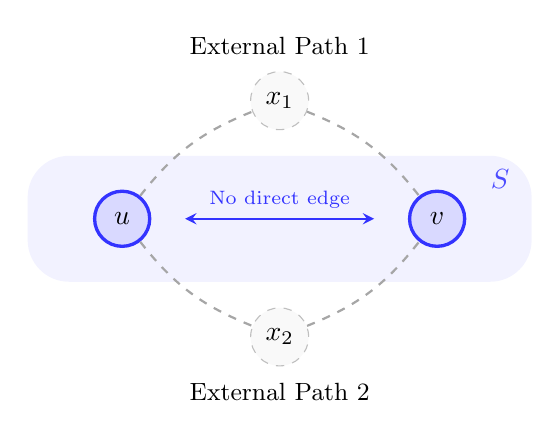
\begin{tikzpicture}[
            vertex/.style={circle, draw=black, thick, minimum size=6mm, inner sep=0pt},
            s_vertex/.style={circle, draw=blue!80, fill=blue!15, very thick, minimum size=7mm},
            external/.style={circle, draw=gray!50, fill=gray!5, dashed, minimum size=6mm},
            edge/.style={thick},
            ext_edge/.style={thick, dashed, gray!70}
        ]

        % Draw the "S" region background
        \fill[blue!5, rounded corners=15pt] (-1.2,-0.8) rectangle (5.2,0.8);
        \node[blue!70] at (4.8, 0.5) {\textbf{$S$}};

        % Vertices in S
        \node[s_vertex] (u) at (0,0) {$u$};
        \node[s_vertex] (v) at (4,0) {$v$};

        % External vertices
        \node[external] (x1) at (2, 1.5) {$x_1$};
        \node[external] (x2) at (2, -1.5) {$x_2$};

        % Paths through external vertices
        \draw[ext_edge] (u) to[bend left=15] (x1);
        \draw[ext_edge] (x1) to[bend left=15] (v);

        \draw[ext_edge] (u) to[bend right=15] (x2);
        \draw[ext_edge] (x2) to[bend right=15] (v);

        % Annotation for the reader
        \node[align=center, font=\small] at (2, 2.2) {External Path 1};
        \node[align=center, font=\small] at (2, -2.2) {External Path 2};

        % Indicators
        \draw[<->, >=stealth, blue!80, thick] (0.8,0) -- (3.2,0) node[midway, above, font=\scriptsize] {No direct edge};

    \end{tikzpicture}
    \caption{\textbf{Embedded Connectivity vs. Induced Structure.} An illustration of Remark~\ref{rem:cohesive-not-induced} for $c=2$. The set $S = \{u, v\}$ is $2$-cohesive because there exist two internally vertex-disjoint $u$--$v$ paths in $G$. However, since these paths traverse vertices $x_1, x_2 \in V \setminus S$, the induced subgraph $G[S]$ remains disconnected. This highlights that $c$-cohesiveness captures how a set is \textit{robustly anchored} within the global graph topology rather than its internal density.}
    \label{fig:embedded_connectivity}
\end{figure}


\begin{figure}[ht]
    \centering
    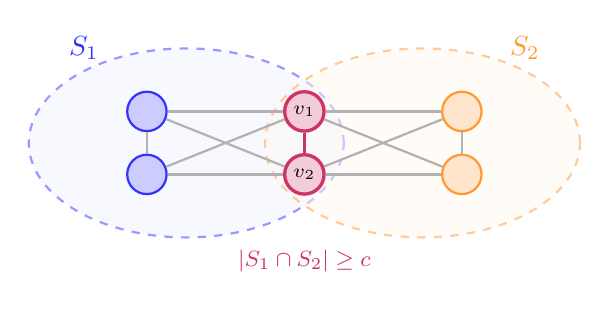
\begin{tikzpicture}[
            vertex/.style={circle, draw=black, thick, minimum size=5mm, inner sep=0pt, font=\scriptsize},
            s1_node/.style={fill=blue!20, draw=blue!80},
            s2_node/.style={fill=orange!20, draw=orange!80},
            intersect_node/.style={fill=purple!20, draw=purple!80, very thick},
            edge/.style={thick, gray!60}
        ]

        % Set S1 boundaries (Conceptual)
        \draw[blue!40, dashed, thick, fill=blue!5, fill opacity=0.5] (0.5,0) ellipse (2cm and 1.2cm);
        \node[blue!80] at (-0.8, 1.2) {$S_1$};

        % Set S2 boundaries (Conceptual)
        \draw[orange!40, dashed, thick, fill=orange!5, fill opacity=0.5] (3.5,0) ellipse (2cm and 1.2cm);
        \node[orange!80] at (4.8, 1.2) {$S_2$};

        % Nodes unique to S1
        \node[vertex, s1_node] (a) at (0, 0.4) {};
        \node[vertex, s1_node] (b) at (0, -0.4) {};

        % Nodes in Intersection (c=2)
        \node[vertex, intersect_node] (i1) at (2, 0.4) {$v_1$};
        \node[vertex, intersect_node] (i2) at (2, -0.4) {$v_2$};
        \node[purple!80, font=\footnotesize] at (2, -1.5) {$|S_1 \cap S_2| \ge c$};

        % Nodes unique to S2
        \node[vertex, s2_node] (c) at (4, 0.4) {};
        \node[vertex, s2_node] (d) at (4, -0.4) {};

        % Edges within S1
        \draw[edge] (a) -- (i1); \draw[edge] (a) -- (i2);
        \draw[edge] (b) -- (i1); \draw[edge] (b) -- (i2);
        \draw[edge] (a) -- (b);

        % Edges within S2
        \draw[edge] (c) -- (i1); \draw[edge] (c) -- (i2);
        \draw[edge] (d) -- (i1); \draw[edge] (d) -- (i2);
        \draw[edge] (c) -- (d);

        % Intersection edge
        \draw[edge, purple!80, very thick] (i1) -- (i2);

    \end{tikzpicture}
    \caption{\textbf{The Union Property of Cohesive Sets.} An illustration of Lemma~\ref{lem:union_cohesive} for $c=2$. Two $2$-cohesive sets $S_1$ (blue) and $S_2$ (orange) overlap at a vertex set of size at least $c$ (purple). This overlap ensures that the $c$ internally vertex-disjoint paths required for any pair $u \in S_1, v \in S_2$ are preserved in the union, allowing $S_1 \cup S_2$ to form a single, larger structural component. This property allows the maximal simplex network to remain connected and well-defined.}
    \label{fig:union_property}
\end{figure}

\begin{figure*}[t]
    \centering
    \begin{tikzpicture}[
            scale=1.2,
            vertex/.style={circle, draw=black, fill=white, thick, minimum size=6mm, inner sep=0pt, font=\footnotesize},
            gedge/.style={draw=black!70, thick},
            face/.style={fill opacity=0.4, draw opacity=0.7, line join=round}
        ]

        % ================= PANEL A: THE GRAPH G =================
        \begin{scope}[xshift=0cm]
            \node[font=\bfseries] at (1.1, 2.5) {A) Graph Structure $G$};

            % Coordinates
            \coordinate (v1) at (0, 0);
            \coordinate (v2) at (2.2, 0);
            \coordinate (v3) at (1.1, -0.8);
            \coordinate (v4) at (1.1, 1.8);
            \coordinate (v5) at (1.1, -2.2);

            % Edges (The two K4 clusters)
            \draw[gedge] (v1)--(v2)--(v3)--cycle; % Shared face
            \draw[gedge] (v4)--(v1) (v4)--(v2) (v4)--(v3); % Top K4
            \draw[gedge] (v5)--(v1) (v5)--(v2) (v5)--(v3); % Bottom K4

            % Vertices
            \node[vertex] at (v1) {$v_1$};
            \node[vertex] at (v2) {$v_2$};
            \node[vertex] at (v3) {$v_3$};
            \node[vertex] at (v4) {$v_4$};
            \node[vertex] at (v5) {$v_5$};

            \node[font=\small, gray] at (1.1, -3.0) {Two overlapping $K_4$ sets};
        \end{scope}

        % Transition Arrow
        \draw[-{Stealth[scale=1.5]}, line width=2pt, gray!30] (3.2, 0) -- (4.3, 0);

        % ================= PANEL B: THE COMPLEX DELTA(G) =================
        \begin{scope}[xshift=5.5cm]
            \node[font=\bfseries] at (1.1, 2.5) {B) Cohesive Complex $\Delta(G)$};

            % Coordinates (Mirrored from Panel A)
            \coordinate (s1) at (0, 0);
            \coordinate (s2) at (2.2, 0);
            \coordinate (s3) at (1.1, -0.8);
            \coordinate (t1) at (1.1, 1.8);
            \coordinate (t2) at (1.1, -2.2);

            % 3-Simplex 1 (Blue)
            \fill[blue!40, face] (s1)--(s2)--(t1)--cycle;
            \fill[blue!30, face] (s2)--(s3)--(t1)--cycle;
            \draw[blue!80, thick] (s1)--(t1) (s2)--(t1) (s3)--(t1);

            % 3-Simplex 2 (Orange)
            \fill[orange!40, face] (s1)--(s2)--(t2)--cycle;
            \fill[orange!30, face] (s2)--(s3)--(t2)--cycle;
            \draw[orange!80, thick] (s1)--(t2) (s2)--(t2) (s3)--(t2);

            % Shared 2-Simplex (Separator - Purple)
            \fill[purple!70, opacity=0.8] (s1)--(s2)--(s3)--cycle;
            \draw[purple, very thick] (s1)--(s2)--(s3)--cycle;

            % Redraw vertices
            \node[vertex] at (s1) {$v_1$};
            \node[vertex] at (s2) {$v_2$};
            \node[vertex] at (s3) {$v_3$};
            \node[vertex] at (t1) {$v_4$};
            \node[vertex] at (t2) {$v_5$};

            % Legend/Labeling
            \node[anchor=west, font=\scriptsize, blue!80] at (2.5, 1.0) {Maximal 3-simplex $\sigma_1$};
            \node[anchor=west, font=\scriptsize, orange!90] at (2.5, -1.0) {Maximal 3-simplex $\sigma_2$};
            \node[anchor=west, font=\scriptsize, purple] at (2.5, 0) {Separator $\tau = \sigma_1 \cap \sigma_2$};
        \end{scope}

    \end{tikzpicture}
    \caption{\textbf{From Graph Structure to Cohesive Simplicial Complex.} An illustration of Definition~\ref{def:cohesive-complex}. \textbf{(A)} A graph $G$ consisting of two $K_4$ cliques sharing a common $K_3$ face defined by vertices $\{v_1, v_2, v_3\}$. \textbf{(B)} The geometric realization of the cohesive simplicial complex $\Delta(G)$. The vertex sets of the two $K_4$s constitute minimal $3$-cohesive sets, which form the maximal simplices (the blue and orange tetrahedra) of the complex. Their intersection, the triangle $\{v_1, v_2, v_3\}$ (highlighted in purple), is a minimal $2$-cohesive set that acts as a separator. This visualization demonstrates how $\Delta(G)$ encodes the multi-scale connectivity of $G$ into a unified topological structure.}
    \label{fig:cohesive_complex}
\end{figure*}

\begin{figure*}[t]
    \centering

    \begin{tikzpicture}[
            node distance=2cm and 2.5cm,
            % Style for Maximal Simplices (The "Meat" of the graph)
            maxsimplex/.style={
                    circle,
                    draw=orange!90,
                    fill=orange!10,
                    very thick,
                    minimum size=1.8cm,
                    align=center,
                    font=\small\bfseries,
                    drop shadow={opacity=0.1}
                },
            % Style for Separators (The "Joints" of the graph)
            separator/.style={
                    rounded rectangle,
                    draw=teal!90,
                    fill=teal!10,
                    thick,
                    minimum size=1.2cm,
                    minimum width=2cm,
                    align=center,
                    font=\footnotesize,
                    drop shadow={opacity=0.1}
                },
            % Edge style representing inclusion
            conn_edge/.style={line width=1.5pt, color=gray!60},
            % Background layer styles
            layer_label/.style={font=\sffamily\bfseries\small, gray},
            background_area/.style={rounded corners, fill=gray!5, draw=gray!20, dashed}
        ]

        % --- Positioning Nodes in a Tree Structure ---

        % Level 1: Main trunk Maximal Simplices
        \node[maxsimplex] (s1) at (0,0) {$\sigma_1$\\$\{1,2,3,4\}$};
        \node[maxsimplex] (s2) at (5,0) {$\sigma_2$\\$\{3,4,5,6\}$};
        \node[maxsimplex] (s3) at (10,0) {$\sigma_3$\\$\{5,6,7\}$};

        % Level 2: Separators connecting the main trunk
        % Placed between s1-s2 and s2-s3
        \path (s1) -- (s2) node[midway, separator] (t12) {$\tau_{12}$\\$\{3,4\}$};
        \path (s2) -- (s3) node[midway, separator] (t23) {$\tau_{23}$\\$\{5,6\}$};

        % Level 3: A Branch extending from sigma_2
        % Separator branching down
        \node[separator, below=2cm of s2] (t24) {$\tau_{24}$\\$\{5\}$};
        % Maximal simplex attached to that separator
        \node[maxsimplex, below=2cm of t24] (s4) {$\sigma_4$\\$\{5,8,9\}$};


        % --- Drawing Edges (The Bipartite Connections) ---
        % Connecting main trunk
        \draw[conn_edge] (s1) -- (t12) -- (s2) -- (t23) -- (s3);
        % Connecting branch
        \draw[conn_edge] (s2) -- (t24) -- (s4);


        % --- Background Layers & Annotations for Clarity ---
        \begin{scope}[on background layer]
            % Area for Maximal Simplices
            \node[background_area, fit=(s1)(s3)(s4), label={[layer_label, anchor=south west]north west:Node Class 1: Maximal Simplices ($\sigma_i$)}] (layer1) {};

            % Area for Separators
            \node[background_area, fit=(t12)(t23)(t24), label={[layer_label, anchor=south west]north west:Node Class 2: Minimal Separators ($\tau_j$)}] (layer2) {};
        \end{scope}

        % Add an arrow indicating the inclusion relationship
        \node[anchor=east, font=\footnotesize, gray!80, align=right] at (-1.5, -3) {Edges represent inclusion:\\$\tau \subset \sigma$};
        \draw[->, thick, gray!60, bend right] (-1.5, -3.2) to (t24);

    \end{tikzpicture}

    \caption{\textbf{The Maximal Simplex Network: A Tree-Structured Representation.} An illustration of the bipartite graph defined in Definition~\ref{def:maximal_simplex_network}. The network consists of two node classes: maximal simplices of $\Delta(G)$ (orange circles) and their intersections acting as minimal separators (teal rounded rectangles). An edge exists if a separator is a proper face of a maximal simplex (e.g., $\tau_{12}=\{3,4\}$ is contained in $\sigma_1=\{1,2,3,4\}$). As guaranteed by Lemma~\ref{lem:maximal_simplex_network_acyclic}, this structure is acyclic, forming a tree that hierarchically decomposes the graph's cohesive structure. This tree acts as a robust graph invariant for isomorphism testing.}
    \label{fig:maximal_simplex_network}
\end{figure*}
